\documentclass[12pt,a4paper,oneside]{article}
\title{作业1-HTML_Parser}
\usepackage{ctex}
\usepackage{amsmath,amscd,amsbsy,amssymb,latexsym,url,bm,amsthm}
\usepackage{epsfig,graphicx,subfigure}
\usepackage{enumitem,balance}
\usepackage{wrapfig}
\usepackage{mathrsfs,euscript}
\usepackage[usenames]{xcolor}
\usepackage{hyperref}
\usepackage[vlined,ruled,commentsnumbered,linesnumbered]{algorithm2e}
\usepackage{float}
\usepackage{geometry}
\usepackage{listings}

\geometry{a4paper,scale=0.8}


\title{Lab2 \quad Crawler-1}
\date{2021.9}
\author{孙济宸\quad \quad 学号:520030910016 \quad  \quad 班级:F2003003}
\begin{document}
\maketitle
\section{实验概览}
\begin{enumerate}
	\item 通过urllib的opener、request等方法发送含有账号密码数据等请求并获取cookie模拟登陆,并且解析账户信息页获取账户信息。
	\item 通过实现url加入队列的不同方式,模拟dfs/bfs爬取网页树并获取链接拓扑图的操作。
	\item 利用(2)中的bfs/dfs方式,对网页解析其所含对全部超链接后进行广度/深度优先爬取。
\end{enumerate}
\section{实验环境}
\begin{itemize}
	\item Docker
	\item beautifulsoup (bs4)
	\item urllib, urllib.parse, urllib.request
	\item re
\end{itemize}
\section{练习题的解决思路}
\subsection{问题1}
先使用cookiejar、HTTPCookieProcessor构建opener,并添加headers;然后使用request向登陆页面发送包含账号密码的请求,并保存登陆后的cookie;再用opener打开账户信息页面,并解析html获得账号信息。
\subsection{问题2}
对于每个网页,其中大多都含有许多指向其他网页的url,这样网页-子页-子页的子页\dots 就可以形成树。
众所周知,树有bfs/dfs遍历,区别就是对网页中找到的url(子页),使用FIFO队列/FILO(栈)。只要控制队列的插入位置就能实现bfs和dfs了。


\begin{lstlisting}[language={Python},numbers=left,numberstyle=\tiny,%frame=shadowbox, rulesepcolor=\color{red!20!green!20!blue!20},  
   keywordstyle=\color{blue!70!black},  
   commentstyle=\color{blue!90!},  
   basicstyle=\ttfamily]  
def union_dfs(a, b):
    for e in b:
        if e not in a:
            a.append(e)    # 元素入栈(FILO)


def union_bfs(a, b):
    for e in b:
        if e not in a:
            a.insert(0,e)   # 元素入队(FIFO)
\end{lstlisting}  





\subsection{问题3}

使用Lab1中获取网页中所有url的函数(匹配所有<a href="...">的标签 ),以(2)中dfs、bfs获取新url的方式即可完成网页树的爬取。
需要注意的是,爬取到的url可能是无效链接,需要注意异常处理(try catch);此外文件IO方面,获取的页面需要用特定编码解码,保存html时应该限制文件名长度。
\begin{lstlisting}[language={Python},numbers=left,numberstyle=\tiny,%frame=shadowbox, rulesepcolor=\color{red!20!green!20!blue!20},  
   keywordstyle=\color{blue!70!black},  
   commentstyle=\color{blue!90!},  
   basicstyle=\ttfamily]  
def get_page(page,coding = 'utf-8'):
    
    try:
        content = urllib.request.urlopen(page,timeout=TIMEOUTSECONDS).read()
    except:
        raise ValueError
    else:
        return content.decode(coding) # 用指定的编码方式解码,防止html乱码
        
def crawl(seed, method, max_page):
    tocrawl = [seed]
    crawled = []
    graph = {}
    count = 0

    while tocrawl and count < max_page:
        page = tocrawl.pop()
        if page not in crawled and page:
            #print("current page:",page)
            try:
                content = get_page(page)
            except ValueError:
                print(page,"not found or cannot open!")
                continue
            else:
                print(page)
           
            add_page_to_folder(page, content)
            outlinks = get_all_links(content, page)
            graph[page] = outlinks
            globals()['union_%s' % method](tocrawl, outlinks)
            crawled.append(page)

            count += 1

    return graph, crawled
\end{lstlisting}  

爬取到的全部html写入文件,并且存储url树的结构。
\section{代码运行结果}
\subsection{问题1结果}
\begin{figure}[H]
	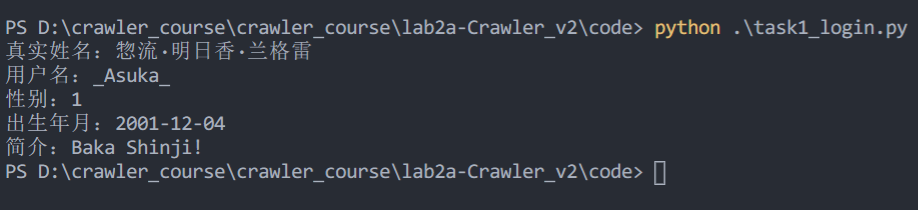
\includegraphics[scale=0.8]{1.png}
	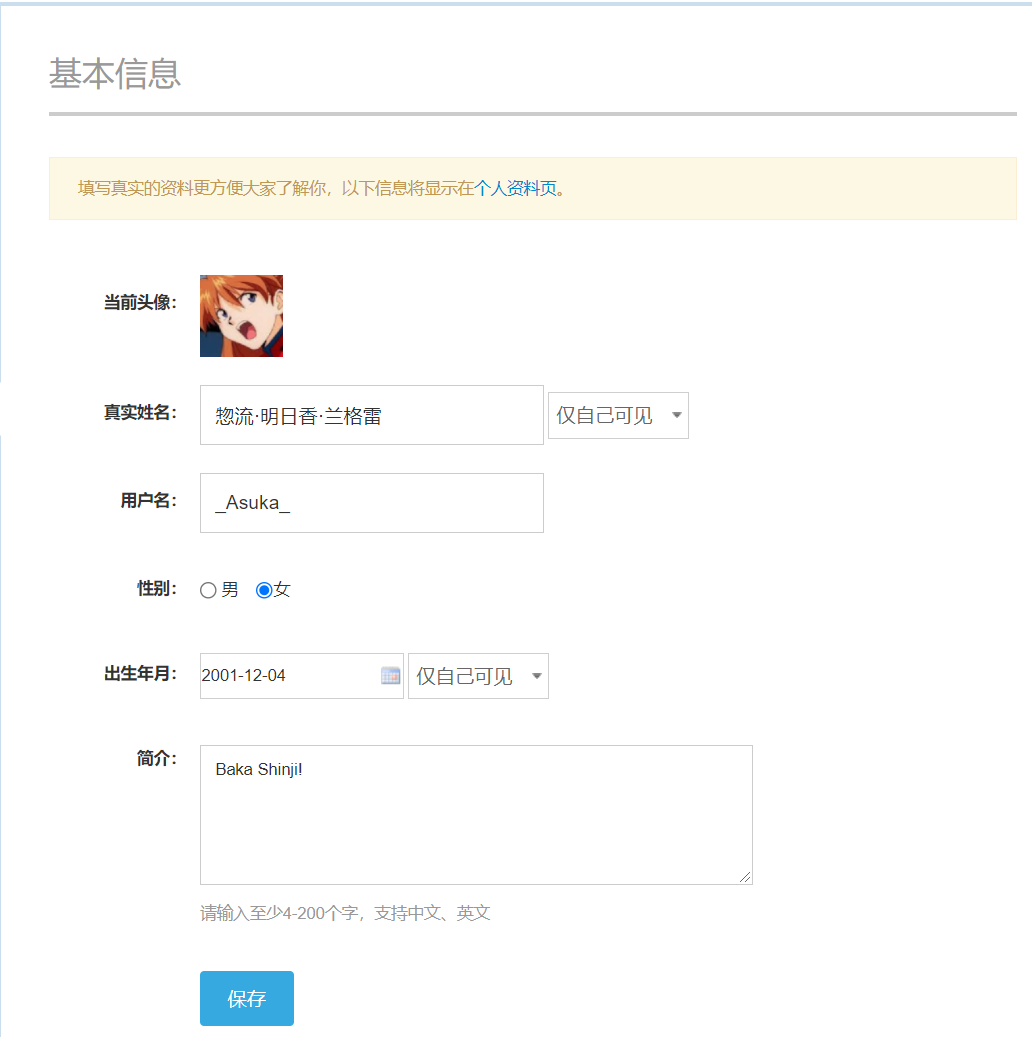
\includegraphics[scale=0.6]{1_1.png}
	 \caption{task1-模拟登陆获用户取信息}
\end{figure}
\let\cleardoublepage\clearpage
\subsection{问题2结果}
\begin{figure}[H] \centering
	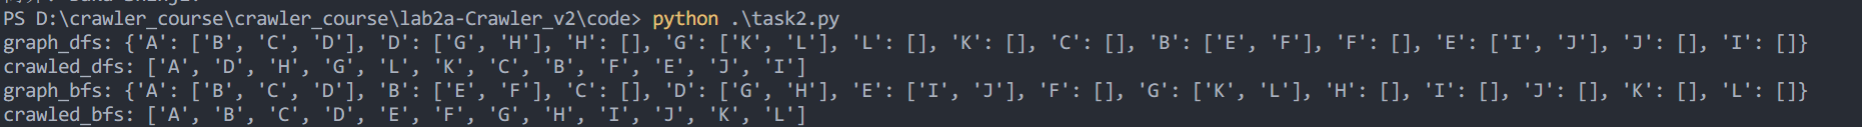
\includegraphics[scale=0.45]{2.png}
	 \caption{task2-bfs、dfs 遍历树}
\end{figure}
\let\cleardoublepage\clearpage
\subsection{问题3结果}
\subsection{BFS}
\begin{figure}[H] \centering
	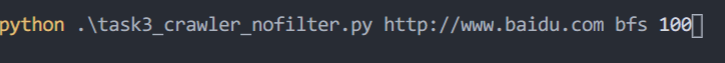
\includegraphics[width=0.6\linewidth]{3_1.png}
	 \caption{BFS}
	 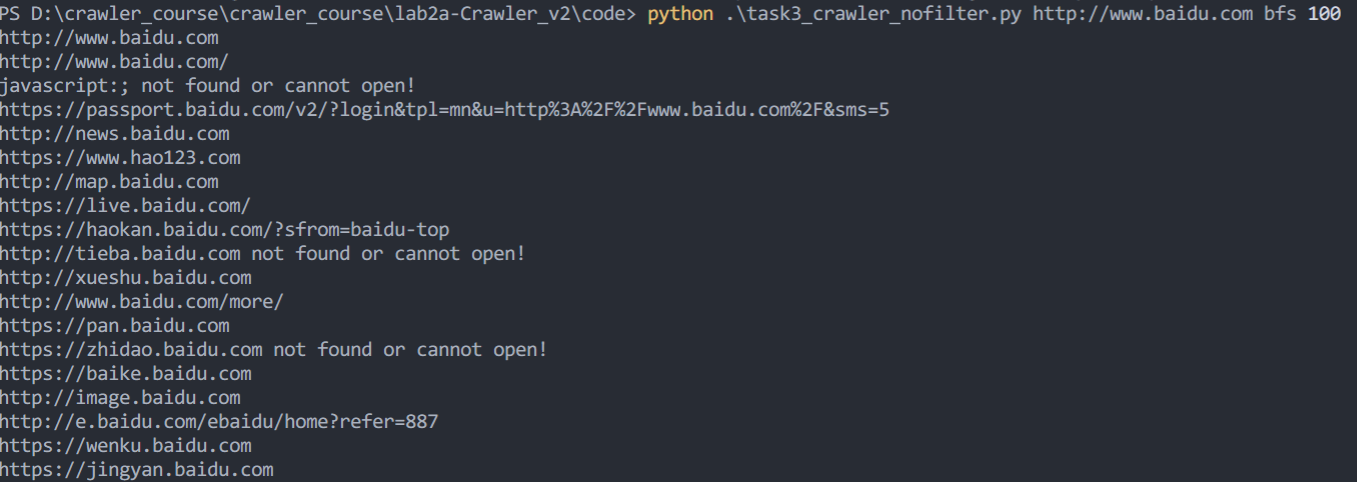
\includegraphics[width=0.6\linewidth]{3_2.png}
	 \caption{BFS}
	 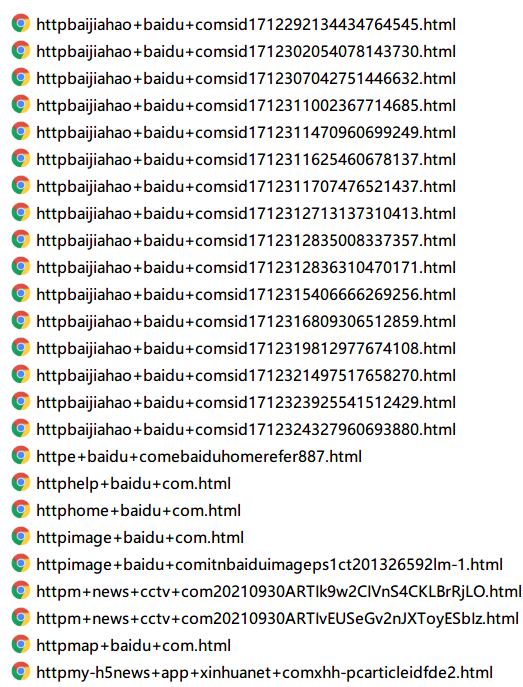
\includegraphics[width=0.6\linewidth]{3_3.png}
	 \caption{html}
	 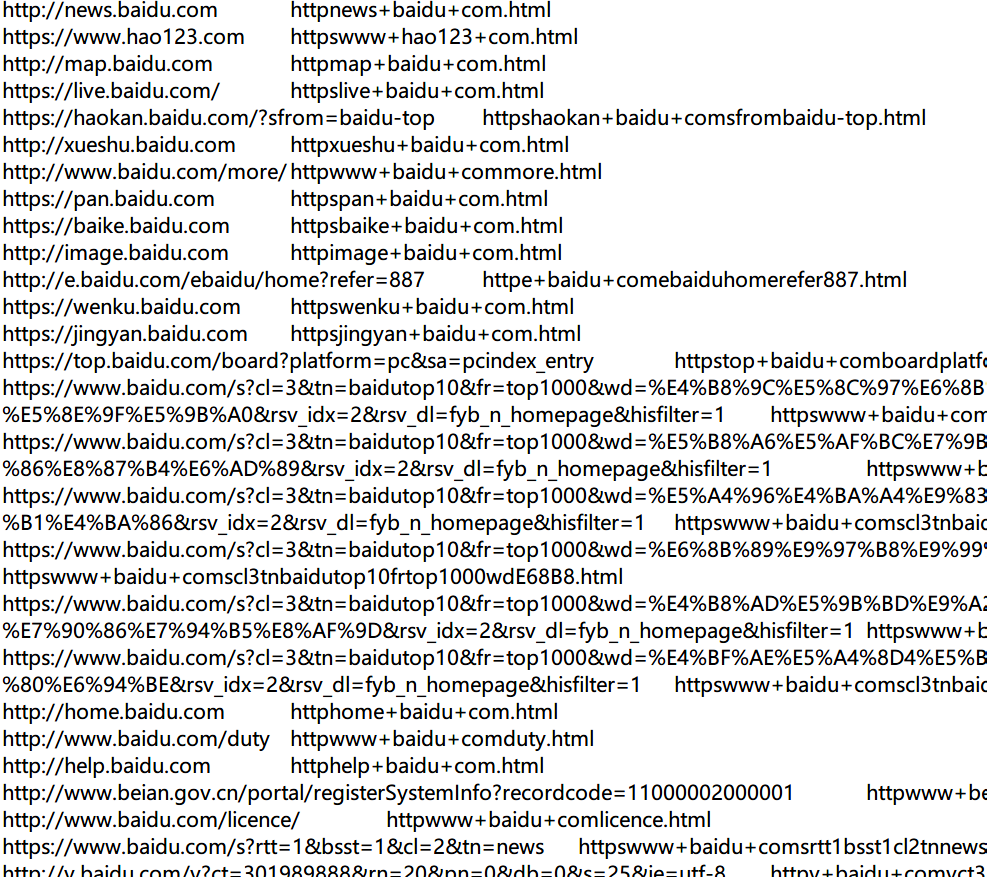
\includegraphics[width=0.6\linewidth]{3_4.png}
	 \caption{index.txt}
\end{figure}
\subsection{DFS}
*由于结果截图过于冗长,省略了html文件和index.txt的截图。
\begin{figure}[H] \centering
	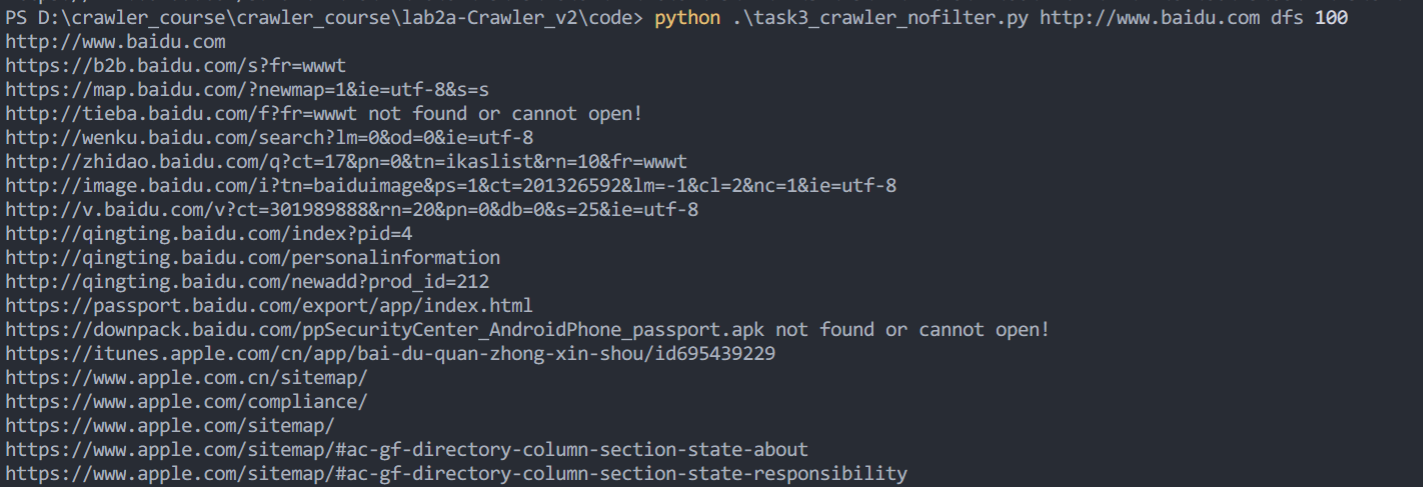
\includegraphics[width=0.6\linewidth]{3_5.png}
	 \caption{DFS}
	
\end{figure}


\section{分析与思考}
\begin{itemize}
	\item Task1中获取用户信息是通过直接向登录页面发送带有账号和密码的请求并且获取cookie实现的。然而现在很多网站都用自己的登录接口,这种方式就无能为力了。
	\item Task2中dfs对python中的list尾部进行操作,但为了统一函数调用,bfs用的是向list头部插元素来模拟FIFO队列,插入是$O(n) (n 为队列中元素个数)$操作,性能开销巨大。实际使用最好把dfs、bfs实现分开实现更好的性能。
	\item Task3中设置timeout是必要的,否则一个无法访问/速度很慢的网页会卡住进程很久
	\item Task3中,必须注意处理catch获取页面的异常;文件的编码问题,大部分网页采用utf-8,读取网页、写入文件时都需要注意编码问题。
	
\end{itemize}
\end{document}

